\section{State of BPMS}
Nowadays \gls{bpms} software supports all stages of \gls{bpm} life-cycle (design, modelling, execution, monitoring and optimization). These systems also offer real-time collaboration, integration with cloud and mobile devices. Many systems also integrate artificial intelligence - for predictive analysis or some automatic decisions. \gls{bpms} software allows to create highly productive application, where is no need to manual implementation of business rules. \gls{bpms} includes defining processes, data models and also user interface. Also highly customized monitoring stage is included. Users can customize \gls{kpi}, look of dashboards and so on.  

\begin{figure}[ht!]
	\centering
    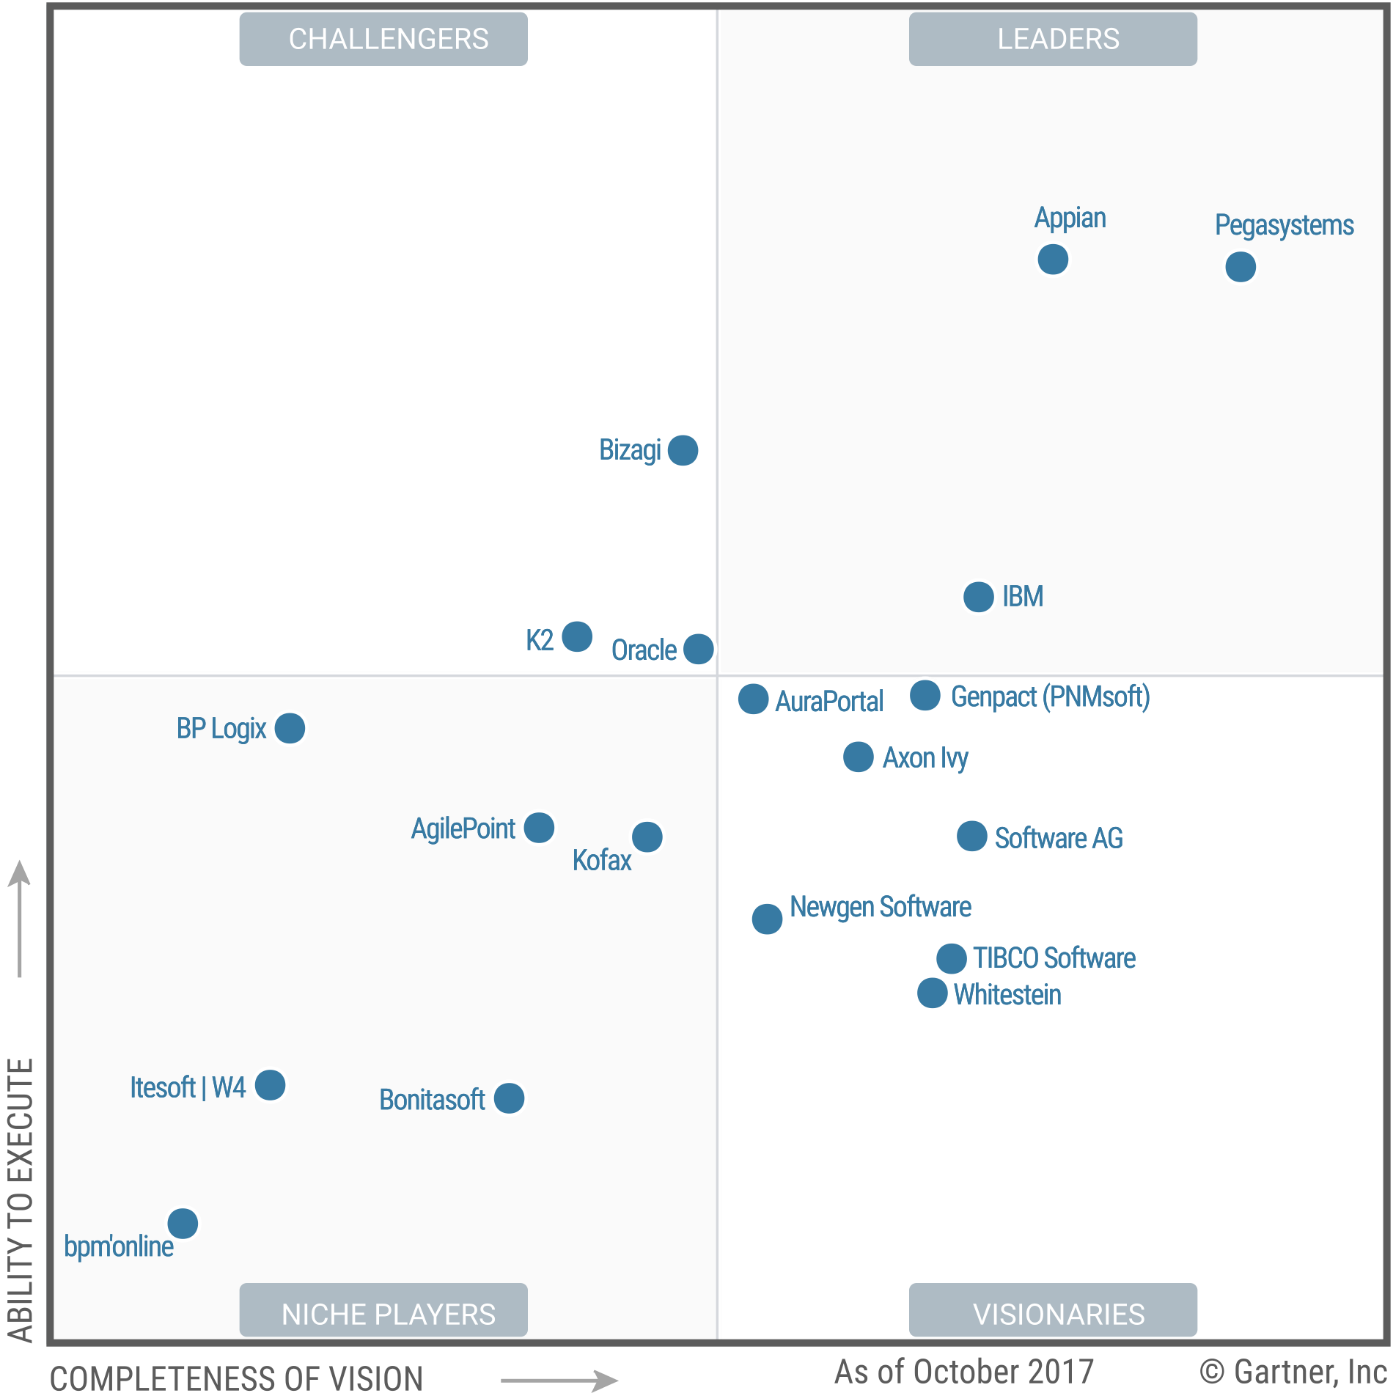
\includegraphics[width=0.6\textwidth, keepaspectratio]{img/gartner-magic-quadrant.png}
    \caption{Gartner Magic Quadrant\cite{gartner-2017} }
    \label{fig:gartner-magic-quadrant}
\end{figure}

Result is typically web based application which employees can use to do their jobs without knowing that there are some defined processes and layer of some BPM software. 

According to \textit{Gartner Magic Quadrant}\cite{gartner-2017}, the most used systems are \textit{Appian}, \textit{Pegasystems}, \textit{IBM} and many more as shown at~\cref{fig:gartner-magic-quadrant}.

 \subsection{Closer look at Process Maker}
 \textit{ProcessMaker} (\href{https://www.processmaker.com/}{https://www.processmaker.com/}) is web-based \gls{bpm} solution which allows to build, run, monitor and optimize business processes. Building of processes is done via \gls{bpmn}. Inside designer (see \cref{fig:process-maker-designer}, users can define data sources (variables) which will be used later within running processes. 
 
 \begin{figure}[ht!]
	\centering
    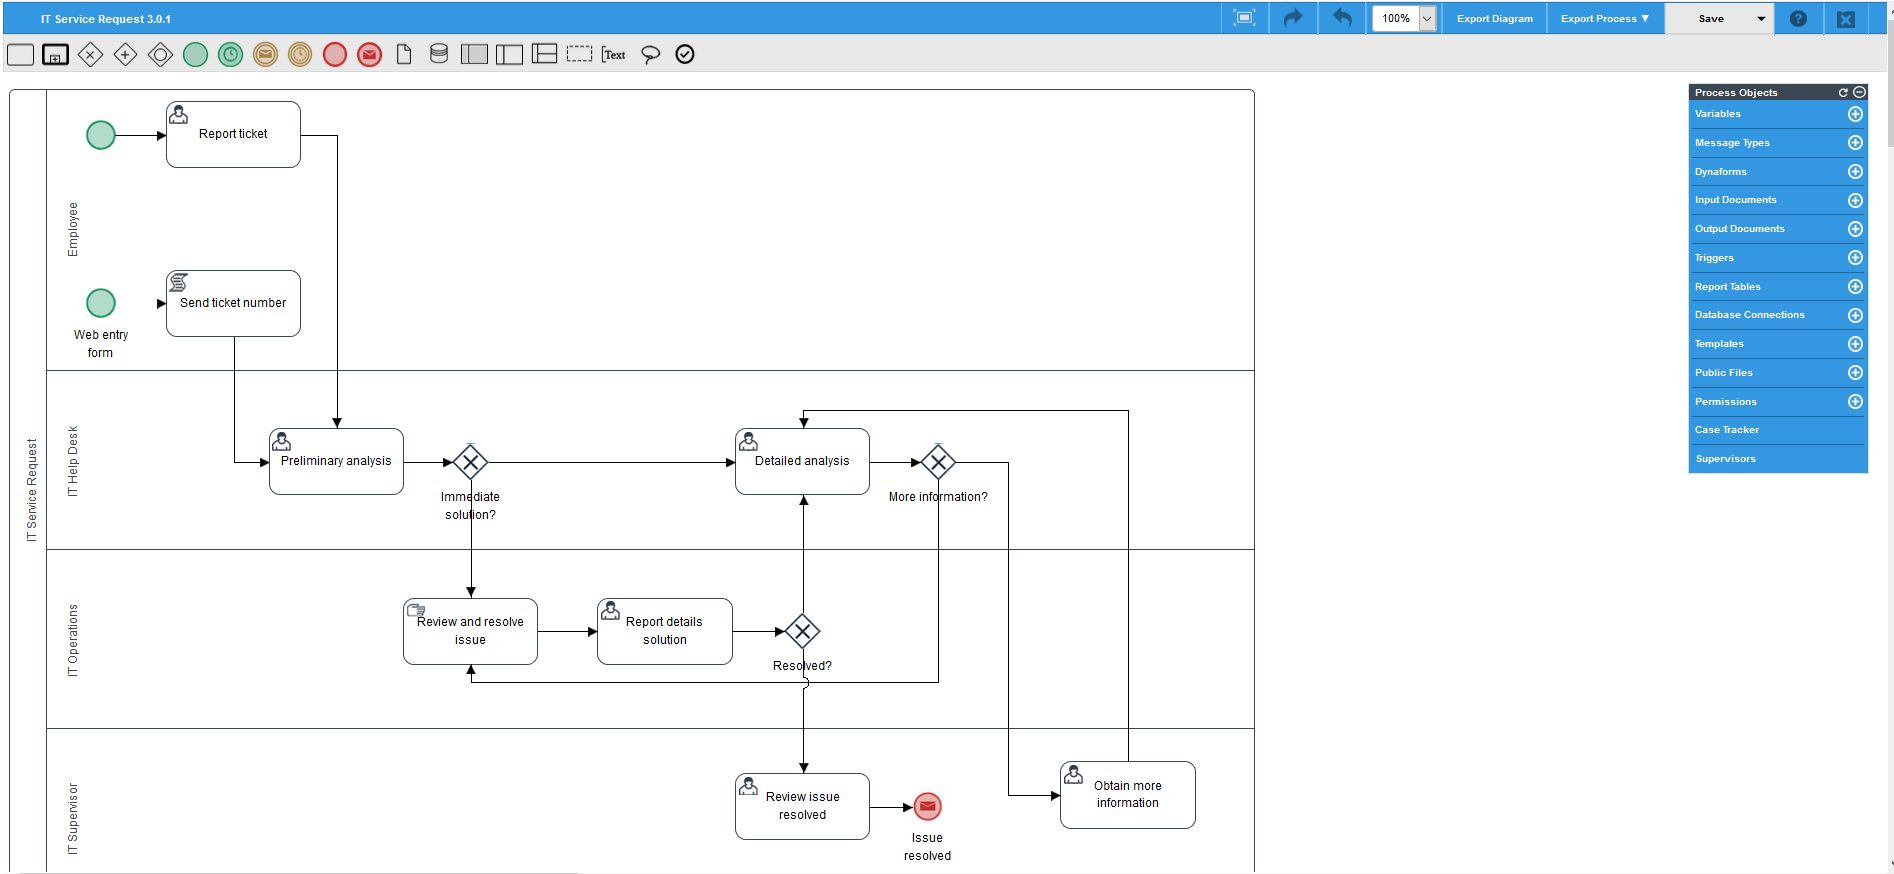
\includegraphics[width=0.8\textwidth, keepaspectratio]{img/process-maker-designer.PNG}
    \caption{ProcessMaker designer}
    \label{fig:process-maker-designer}
\end{figure} 
 
\begin{figure}[ht!]
    \centering
    \subfloat[Dashboard]{{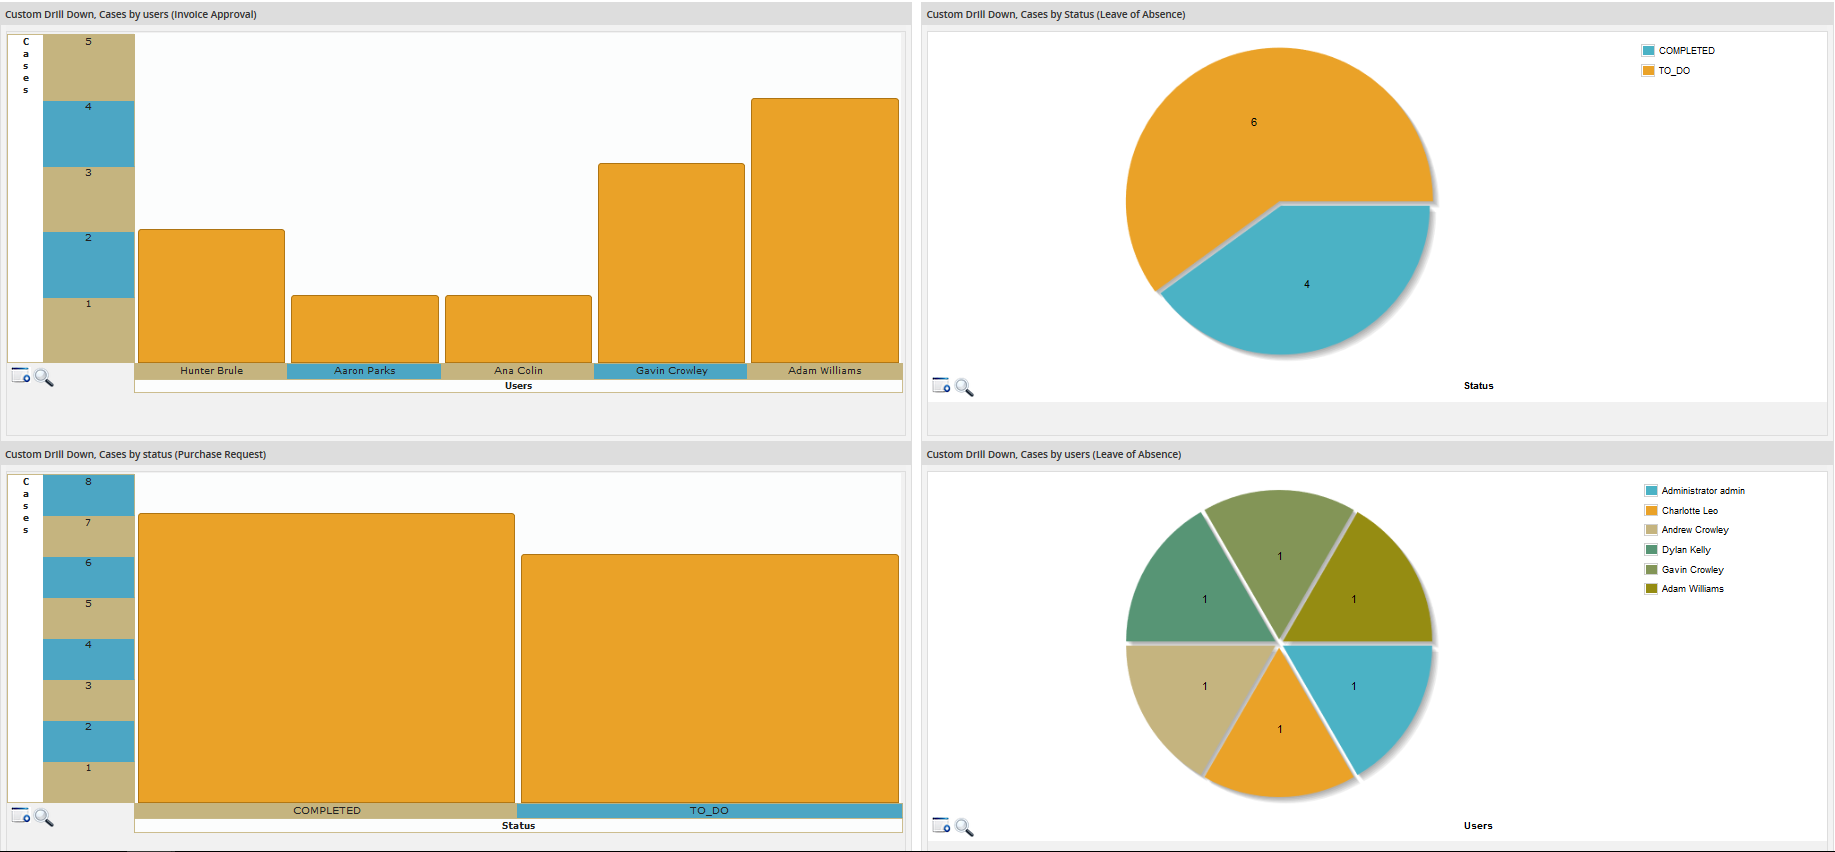
\includegraphics[width=10cm, keepaspectratio]{img/process-maker-dashboard.PNG} }}%
    \qquad
    \subfloat[Employee efficiency KPI]{{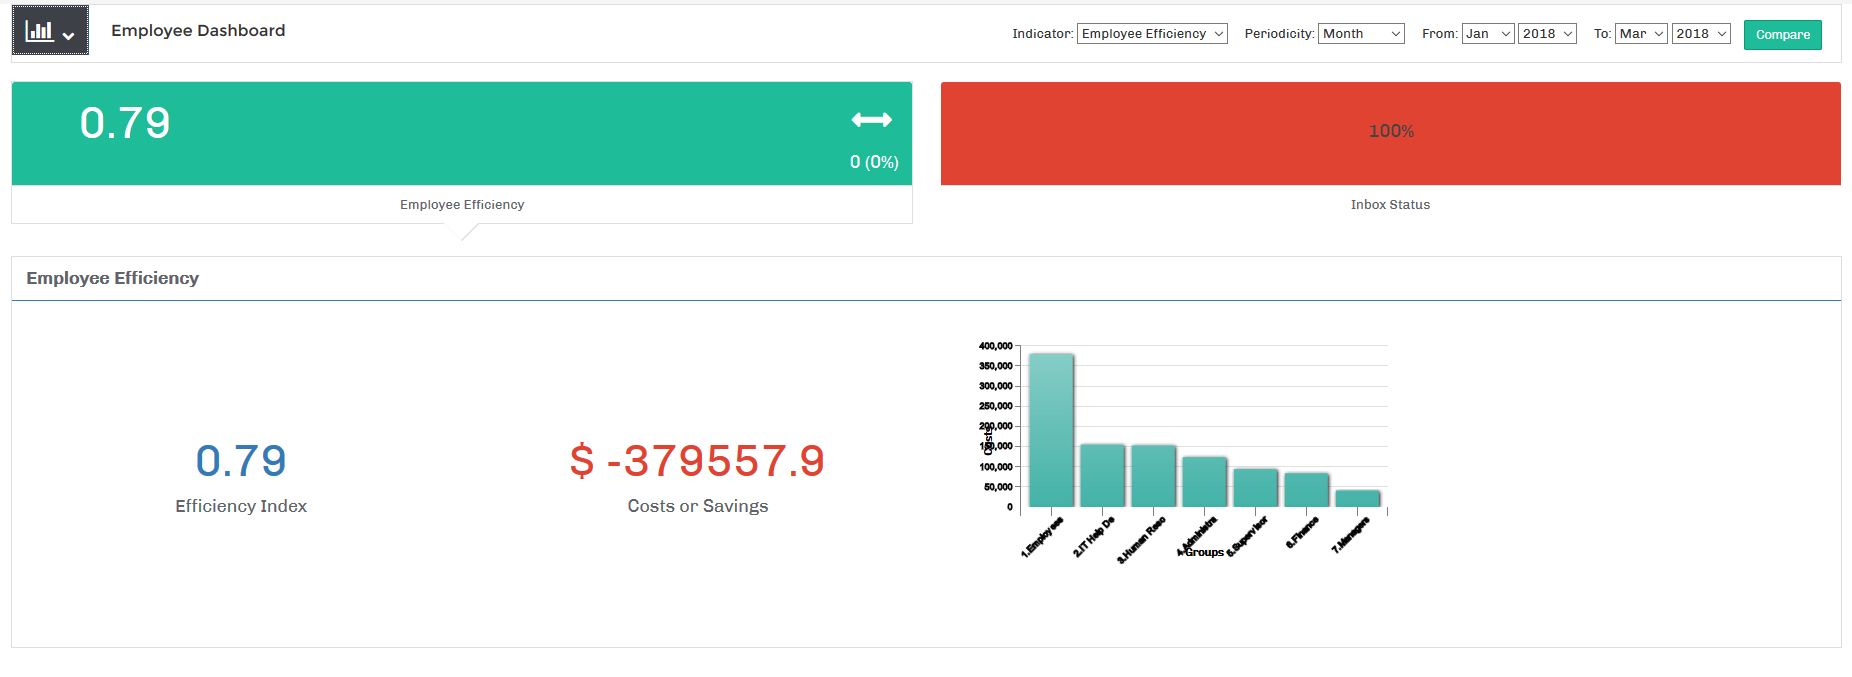
\includegraphics[width=10cm, keepaspectratio]{img/process-maker-employee-kpi.PNG} }}%
    \caption{ProcessMaker dashboard and KPI examples}%
    \label{fig:process-maker-dashboard}%
\end{figure}

 After process is designed and variables defined, next step is to define user interface, called DynaForms. End users interact mainly with \textit{DynaForms}, where they fill appropriate pieces of data. 
 Inside designer of \textit{DynaForms}, user connects data fields with variables from defined processes. Also user can define input or output documents for processes or define events (called triggers) what will happen when some kind of event occurred.
 
 When processes are defined and \textit{DynaForms} created, processes can be deployed. After that, \gls{kpi}s and dashboards can be managed. \textit{ProcessMaker} offers creating custom metrics, which will be precise to business requirements and customize dashboards. Many of graphs are interactive, which can display more detailed information. An example is shown at \cref{fig:process-maker-dashboard}.
 
 From end-user view, \textit{ProcessMaker} (as many others \gls{bpms}) behaves as web-based application, which allows to do his job via predefined \textit{DynaForms}. ProcessMaker moreover offers process map, which is graphical visualisation of running process. Process map is in \gls{bpmn} and each activity element has different colour to indicate its state (\cref{fig:process-maker-process-map}).
 
  \begin{figure}[ht!]
	\centering
    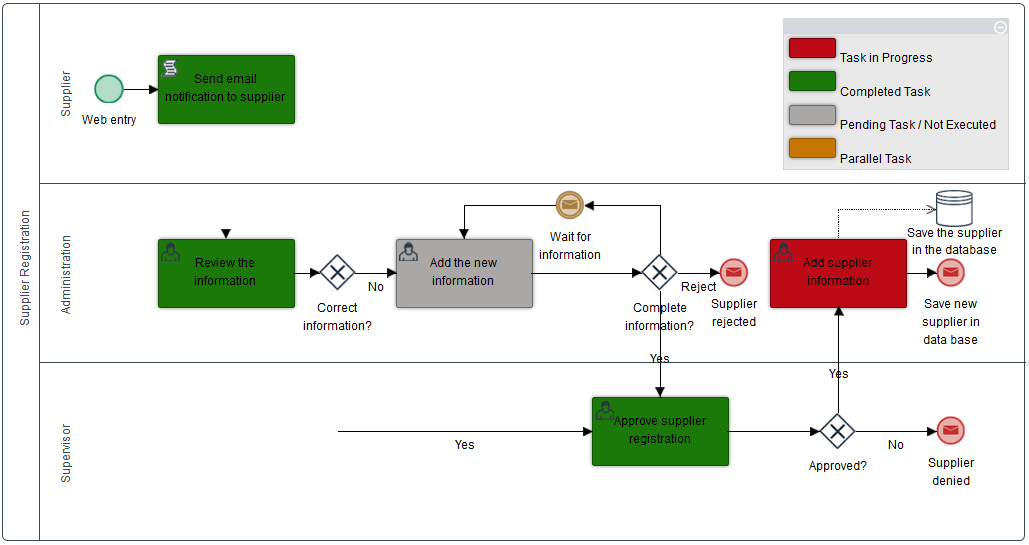
\includegraphics[width=0.8\textwidth, keepaspectratio]{img/process-maker-map.PNG}
    \caption{ProcessMaker process map}
    \label{fig:process-maker-process-map}
\end{figure} 

